\subsection{Integración del \glsentryshort{bmv2} en Mininet-WiFi}
\label{mn-wifi_bmv2_integration}

% Intro
En esta subsección se abordará la integración del \gls{bmv2} en Mininet-WiFi. La integración se ha dividido en tres partes. En las dos primeras se estudiará y analizará, conceptos básicos y desarrollos previos que serán de gran utilidad a la hora de abordar el desarrollo de la interfaz \gls{bmv2} en Mininet-WiFi.

\subsubsection{Análisis de la interfaz \glsentryshort{bmv2} - Mininet}

Desde el equipo de \textit{p4lang} se quiso suministrar un entorno de pruebas donde se pudiera probar los programas P4 desarrollados. El soft-switch donde iban a cargar el programa P4 ya lo tenían, que es el \gls{bmv2}, pero les faltaba una plataforma donde poder desplegar dicho ``switch" e interconectarlo con otras entidades de red. Esta plataforma sería Mininet, una herramienta de emulación de redes.\\
\par

Mininet generalmente se utiliza para emular entornos \gls{sdn} con switches y controladores. Por ello, para lograr la integración de su nuevo switch con los switches ya disponibles en Mininet, tuvieron que añadir una nueva clase llamada \texttt{P4Switch}. Esta nueva clase, heredaría de la clase \texttt{Switch} de Mininet, añadiendo así todos los métodos y atributos necesarios para la orquestación del \gls{bmv2}.\\
\par

Usualmente, cuando se trabaja con Mininet se desarrollan scripts donde se define la topología de la red a emular. En este caso, para brindar de una mayor facilidad a los usuarios de los tutoriales de P4\footnote{\url{https://github.com/p4lang/tutorials}}, las topologías se definen en archivos \texttt{*.json}, los cuales definen toda la topología de red y toda la información del plano de control de cada ``switch" P4. Un ejemplo de dicho archivo pueden encontrarse \href{https://github.com/davidcawork/TFG/blob/master/src/use_cases/p4/case01/scenario/topology.json}{\textbf{aquí}}. De este modo, se consigue abstraer el la definición de la topología del propio script de orquestación de la misma. El script de orquestación de la topología el cual hará uso de la API de Python de Mininet será el script \texttt{run\_exercise.py}, que se puede encontrar \href{https://github.com/davidcawork/TFG/blob/master/src/use_cases/p4/utils/run_exercise.py}{\textbf{aquí}}. De esta manera se tendrá tantos ficheros \texttt{*.json} como topologías se quieran, pero un único script de orquestación.\\
\par

El script \texttt{run\_exercise.py} inicializa un objeto de la clase \texttt{ExerciseRunner} el cual leerá el fichero \texttt{*.json}, procesará la topología con la ayuda de la clase \texttt{ExerciseTopo} y levantará la topología haciendo uso de la API de Python de Mininet. A continuación, en la figura \ref{fig:analysis_p4_wifi_1} se puede apreciar un diagrama UML donde se indica la relación de clases del entrypoint en el levantamiento de los distintos casos de uso.\\
\par

Como ya se comentaba anteriormente, para lograr la integración del \gls{bmv2} en Mininet se tuvo que crear la clase \texttt{P4Switch}. Esta nueva clase, heredaría de la clase \texttt{Switch} de Mininet. A su vez, se crearían nuevas clases hijas de la clase \texttt{P4Switch}, la más importante \texttt{P4RuntimeSwitch} la cual se utilizaría para configurar dicho ``switch" vía P4Runtime. Si se desea ver una vista más amplia de esta relación de clases, ir a la figura \ref{fig:analysis_p4_wifi_2}.

\newpage

% uml_1
% figura escenario
\begin{figure}[ht]
    \centering
    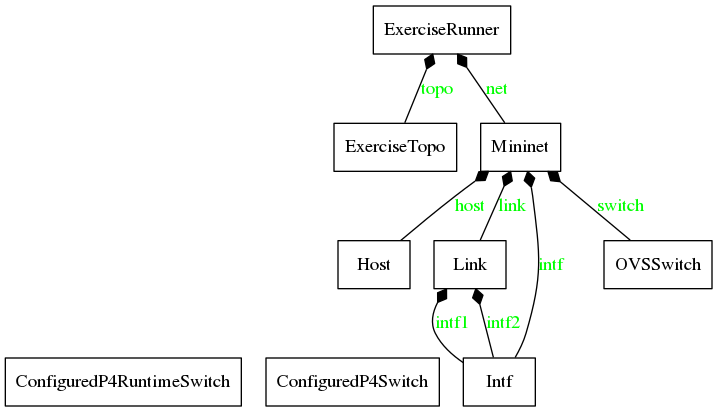
\includegraphics[width=13cm]{archivos/img/dev/p4-wifi/analysis/run_exercise_pertenencia.png}
    \caption{UML del punto de entrada de la interfaz BMv2 - Mininet}
    \label{fig:analysis_p4_wifi_1}
\end{figure}

%uml_2
% figura escenario
\begin{figure}[h!]
    \centering
    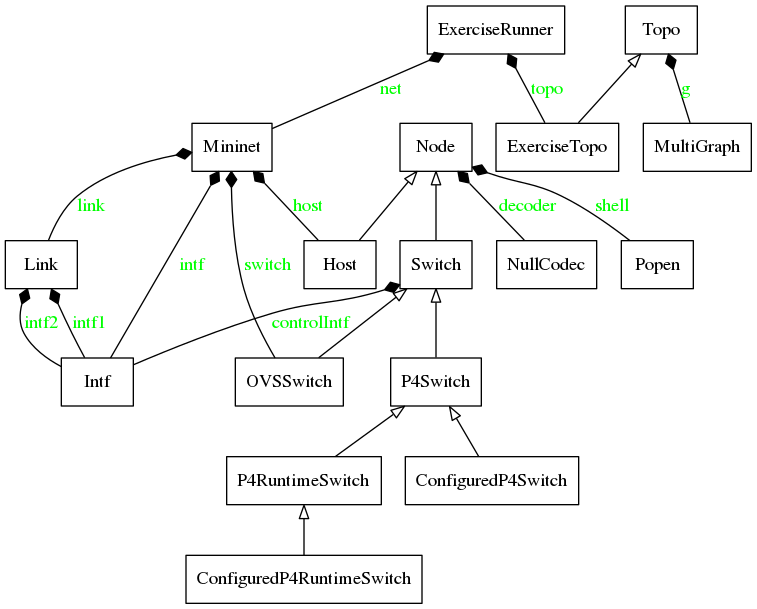
\includegraphics[width=13.5cm]{archivos/img/dev/p4-wifi/analysis/run_exercise_class_names_only.png}
    \caption{UML interfaz BMv2 - Mininet}
    \label{fig:analysis_p4_wifi_2}
\end{figure}



\subsubsection{Análisis del funcionamiento interno de Mininet-WiFi}

Una vez que se revisó el funcionamiento interno de la API de Mininet-P4, se da paso a analizar Mininet-WiFi en profuncidad. Como se comentaba en el capítulo \ref{estadoArte}, Mininet-WiFi es una herramienta de emulación de redes wireless que ha nacido de Mininet, es decir es un fork de este. Al ser un fork comparte gran parte de la jerarquía de clases así como su capacidad para simular ciertos elementos de la red. Aun así, si bien se ha mencionado en numerosas ocasiones que Mininet-WiFi esta desarrollado a partir de Mininet, la capacidad de emulación de interfaces \textit{Wireless} la toma de subsistema wireless de Linux.\\
\par

La arquitectura de virtualización empleada en Mininet-WiFi funciona de forma similar a la Mininet; se hace uso de la herramienta \texttt{mnexec}\footnote{\url{https://github.com/intrig-unicamp/mininet-wifi/blob/master/mnexec.c}} para lanzar distintos procesos de bash en nuevas \textit{Network Namespaces}, uno por cada nodo independiente de la red. De estos procesos colgarán todos los procesos relativos a los distintos nodos de la red. Cuando la emulación haya terminado, se matarán dichos procesos de bash, consiguiendo que no haya ninguna condición de referenciación de las \textit{Network Namespaces}, y estas sean eliminadas por el Kernel.\\
\par

De esta manera, los nodos de la red ya estarían aislados entre sí, por loque lo único que quedaría por virtualizar son las capacidades \textit{wireless} de los nodos que las requieran. Para ellos se hará uso del subsistema \textit{wireless}  del Kernel de Linux, más concretamente el módulo \texttt{mac80211\_hwsim} el cual creará las interfaces \textit{wireless}  en nuestro equipo. Este módulo se comunicará con framework \texttt{mac80211} el cual proveerá de las capacidades de gestión de acceso al medio de la interfaz \textit{wireless} . Además, en el espacio de Kernel aun hay un bloque más, llamado cfg80211, el cual servirá de API para la configuración de las cabeceras 802.11. Esta configuración puede ser realizada por la interfaz netlink de espacio de usuario llamada nl80211. Para la configuración de los puntos de acceso, se hará uso del programa \texttt{HostApd} el cual indicándole la configuración del punto de acceso y la interfaz sobre la cual debe correr, emulará el funcionamiento de un punto de acceso estándar. En la  figura \ref{fig:analysis_p4_wifi_3} se puede ver de manera resumida la arquitectura básica de Mininet-WiFi.\\
\par

% foto arch Mininet-wifis
% figura escenario
\begin{figure}[ht]
    \centering
    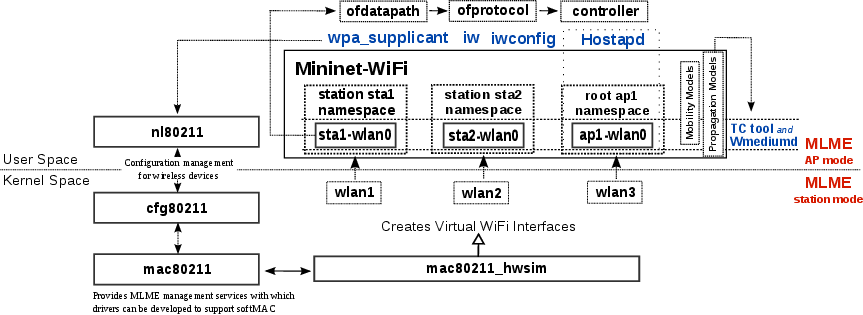
\includegraphics[width=15cm]{archivos/img/dev/p4-wifi/analysis/mininet_wifi_components.png}
    \caption{Arquitectura Mininet-WiFi \cite{7367387}}
    \label{fig:analysis_p4_wifi_3}
\end{figure}


En cuanto a la jerarquía de clases,únicamente cabe mencionar que es bastante similar a la de Mininet. Por destacar dos clases claves en la jerarquía de Mininet-WiFi, serían Node\_Wifi, de la cual heredan todos los nodos con capacidades wireless que posee Mininet-WiFi y por último, la clase IntfWireless, de la cual heredan todos los tipos de enlaces disponibles de Mininet-WiFi (Bajo el estándar \texttt{ieee80211}). A continuación,  en la figuras \ref{fig:analysis_p4_wifi_4} y \ref{fig:analysis_p4_wifi_5}, se indican los UML referentes a dichas clases.\\
\par

% uml_3 wifis
% figura escenario
\begin{figure}[ht]
    \centering
    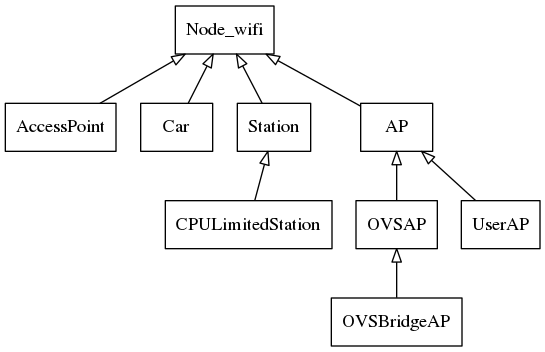
\includegraphics[width=8cm]{archivos/img/dev/p4-wifi/analysis/uml_node.png}
    \caption{UML sobre las relaciones de las clases de tipo Nodo.}
    \label{fig:analysis_p4_wifi_4}
\end{figure}



Como se puede apreciar en los esquemas UML, se ha conseguido aislar la funcionalidad común en las clases padres, con la finalidad de optimizar la cantidad de código de las clases hijas. De esta forma, añadir nuevos tipos de enlaces y nodos en Mininet-WiFi resulta bastante asequible.\\
\par

% uml_4 wifis
% figura escenario
\begin{figure}[ht]
    \centering
    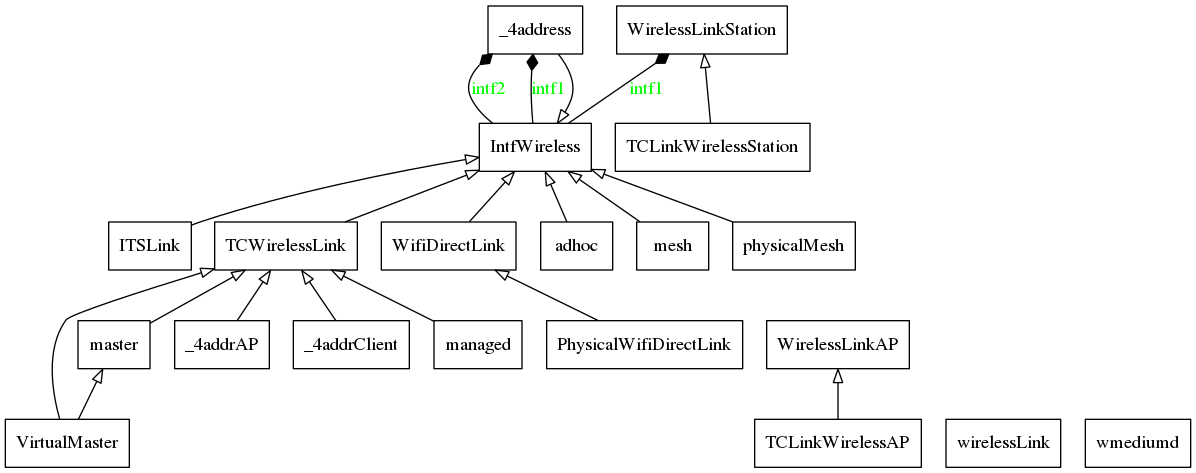
\includegraphics[width=15cm]{archivos/img/dev/p4-wifi/analysis/uml_link.png}
    \caption{UML sobre las relaciones de las clases de tipo Interfaz.}
    \label{fig:analysis_p4_wifi_5}
\end{figure}



\vspace{1cm}
\textbf{Linux Wireless Subsystem}\\
\par

El subsistema \textit{wireless} de Linux consiste en un set de varios módulos que se encuentran en el Kernel de Linux. Estos manejan la configuración del hardware bajo el estándar \texttt{ieee80211}, además de la gestión de la transmisión y la escucha de los paquetes de datos. Yendo de desde abajo hacia arriba en la arquitectura del subsistema, el primer bloque que se encuentra es el módulo mac80211\_hwsim. Este módulo como ya se comentaba es el responsable de crear las interfaces \textit{wireless} virtuales en Mininet-WiFi.\\
\par

% arch LWS
% figura escenario
\begin{figure}[ht]
    \centering
    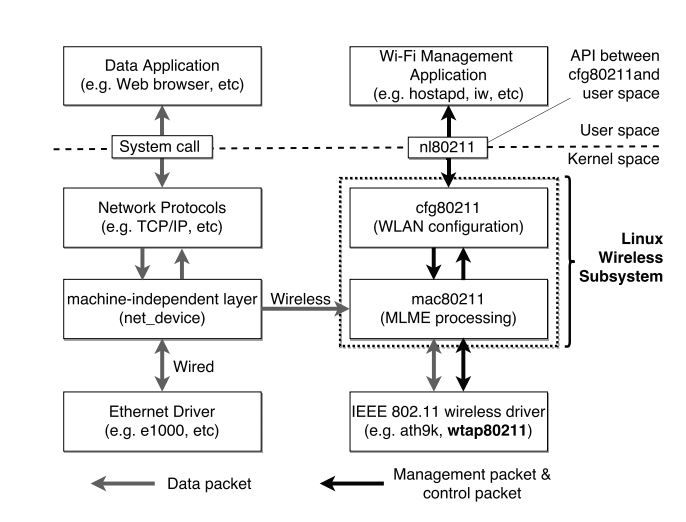
\includegraphics[width=14cm]{archivos/img/dev/p4-wifi/analysis/linux_wireless_subsystem.JPG}
    \caption{Arquitectura del subsistema Wireless de Linux \cite{8330098}}
    \label{fig:analysis_p4_wifi_6}
\end{figure}

El objetivo principal de este módulo mac80211\_hwsim es facilitar a los desarrolladores de drivers de tarjetas \textit{wireless} la prueba de su código e interacción con el siguiente bloque llamado mac80211. Las interfaces virtualizadas no tienen ciertas limitaciones, es decir, a diferencia del hardware real, resulta más sencillo la creación de distintas pruebas con distintas configuraciones sin estar cohibidos por falta de recursos materiales. Este módulo generalmente recibe un único parámetro, que es el número de ``radios", interfaces virtuales, a virtualizar. Dado que las posibilidades que ofrece este módulo eran un poco reducidas, muchos \textit{wrappers} (``envoltorios al software original") han sido creados para ofrecer más funcionalidad a parte de la dada por el propio módulo. La mayoría de herramientas creadas hacen uso de la librería Netlink para comunicarse directamente con el subsistema en el Kernel y así conseguir configuraciones extra, como pueden ser añadir un \gls{rssi} o darle nombre a la interfaz. Un ejemplo de dichas herramientas sería la herramienta \texttt{mac80211\_hwsim\_mgmt}, la cual es usada por Mininet-WiFi para gestionar la creación de las interfaces \textit{wireless} en cada nodo que las requiera.\\
\par

Es importante mencionar el cambio de paradigma que existe en el subsistema \textit{wireless} de Linux con el concepto de interfaz. Generalmente se está acostumbrado a pensar en el concepto de interfaz como un elemento que gestiona el acceso al medio, capa dos, y el propio hardware, capa física, un ejemplo de ello sería una interfaz de Ethernet. Bien, pues en el subsistema wireless se desglosa la interfaz en dos capas \cite{8330098}. Una de ellas es la capa física (\textit{PHY}) donde se puede gestionar por ejemplo en que canal está escuchando la tarjeta wireless emulada. La otra capa es el acceso al medio, representado por las interfaces virtuales que ``cuelgan" de una tarjeta wireless.\\
\par
 La idea detrás de este paradigma, es que puede tener \textit{N} interfaces virtuales asociadas a la misma tarjeta WiFi emulada, lo que resultó sorprendente es que las interfaces virtuales funcionan principalmente con Ethernet (dejando de lado las que están en modo monitor).

\vspace{0.5cm}
\textbf{Limitaciones encontradas}\\
\par
\label{limitacionesEncontradas}

Como ya se ha comentado, la mayoría de interfaces virtuales asociadas a una tarjeta wireless emulada son del tipo de Ethernet, por lo que todos los paquetes que llegan vienen con cabeceras Ethernet. Esto supone una limitación ya que en los casos de uso se quería gestionar las cabeceras WiFi, pero si todas las interfaces virtuales son generalmente del de tipo Ethernet, no será posible.

% foto downstream
% figura escenario
\begin{figure}[ht]
    \centering
    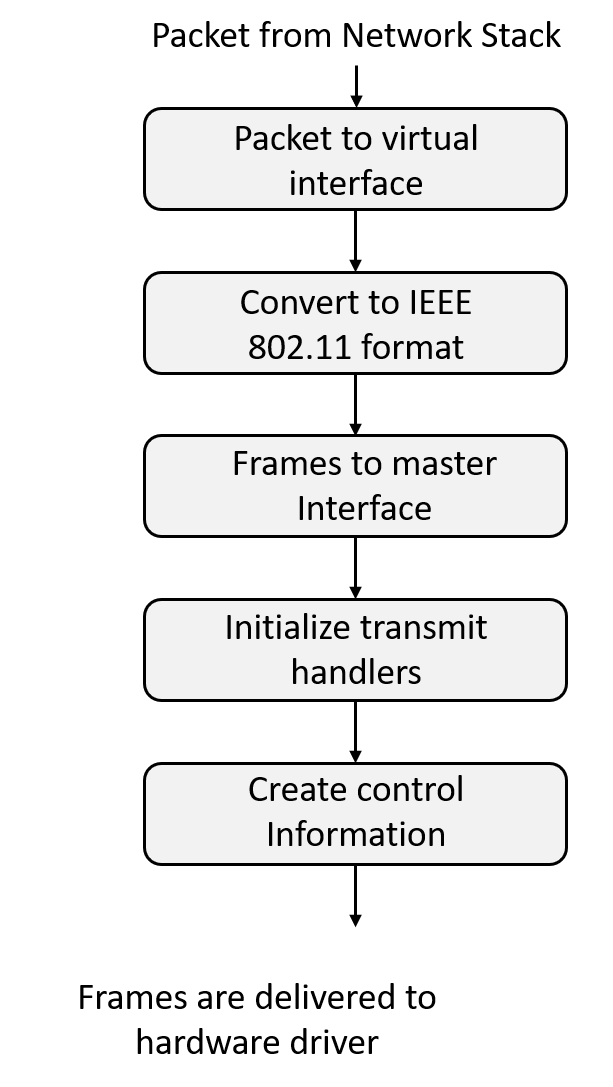
\includegraphics[width=4cm]{archivos/img/dev/p4-wifi/analysis/linux_wireless_subsystem_tx.png}
    \caption{Flujo para la transmisión con el módulo mac80211\_hwsim \cite{5415877}}
    \label{fig:analysis_p4_wifi_7}
\end{figure}

Pero, ¿Qué sentido tiene tener convertir las cabeceras WiFi a cabeceras Ethernet? De momento la única razón que se ha encontrado de esta decisión de diseño, es hacer un diseño más sencillo de todos los drivers que operan bajo el módulo mac80211\_hwsim, que convierten a Ethernet y se lo entregan al stack de red para que lo gestione como un paquete más de una red cableada. De esta forma, las aplicaciones que operen a nivel de interfaz serán más extrapolables. 

% foto upstream
% figura escenario
\begin{figure}[ht]
    \centering
    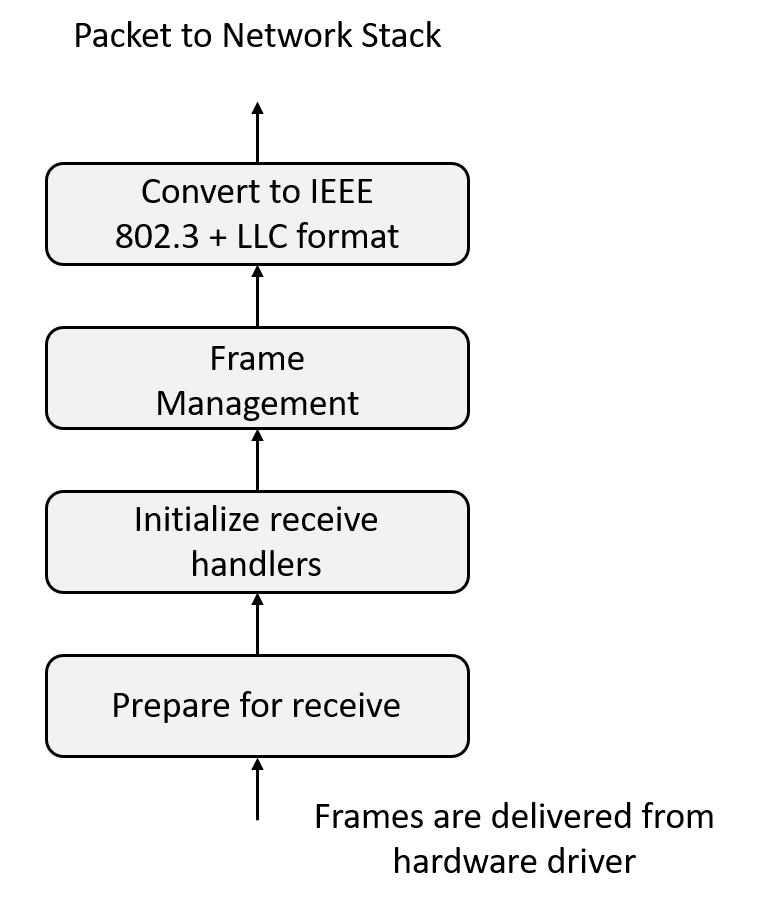
\includegraphics[width=5cm]{archivos/img/dev/p4-wifi/analysis/linux_wireless_subsystem_rx.png}
    \caption{Flujo para la recepción con el módulo mac80211\_hwsim \cite{5415877}}
    \label{fig:analysis_p4_wifi_8}
\end{figure}

Pero, hay que mencionar que esto supone un gasto de recursos considerable, ya que el paquete es encolado hasta tres veces (driver, ethernet queue, qdisc queue) y se tiene que invertir tiempo y recursos en el proceso de traducción de las cabeceras.  \href{https://elixir.bootlin.com/linux/latest/C/ident/__ieee80211_data_to_8023}{\textbf{Aquí}}\footnote{\url{https://elixir.bootlin.com/linux/latest/C/ident/__ieee80211_data_to_8023}} se puede ver la función en el kernel donde se lleva a cabo ese proceso.\\
\par

Esto sucede generalmente y no siempre ya que en el único modo que una interfaz puede llegar a escuchar los paquetes WiFi es en el modo monitor. Pero el modo monitor está pensado únicamente para escuchar paquetes, no para transmitir. Este modo puede ser llevado al limite haciendo una inyección de paquetes (packet injection) por la interfaz.\\
\par

De esta forma se conseguiría el objetivo de manejar las cabeceras WiFi, pero dadas las competencias del \gls{tfg}, este desarrollo se escapa completamente. Ni si quiera Mininet-WiFi, siendo la herramienta de facto para emular redes \textit{wireless}, contempla el manejo de cabeceras WiFi. Por ello, este objetivo se plantea como un desarrollo a posteriori y se mencionará en el trabajo futuro (Ver sección \ref{trabajoFuturo}). \\
\par
El desarrollo pues sobre Mininet-WiFi, consistirá en la integración del \gls{bmv2} en Mininet-WiFi, y probar los casos de uso desarrollados para P4, bajo Mininet-WiFi. Las cabeceras que llegarán a la pipeline serán las de Ethernet, pero como ya se ha explicado, es el propio Kernel quien se encarga de hacer un \textit{casting} de las cabeceras WiFi hacia cabeceras Ethernet.\\
\par

\subsubsection{Desarrollo de la interfaz BMV2 - Mininet-WiFi}

Ahora que ya se tiene una idea sobre el funcionamiento interno de ambas herramientas, vamos a proceder a su integración. A la par que se estaba trabajando en el desarrollo de la integración del \gls{bmv2} en Mininet-WiFi, el investigador Ramon Fontes (desarrollador de la herramienta) abrió un Issue (es decir, una publicación de debate y ampliación de funcionalidad de GitHub) donde se exponía la intención de crear dicha integración. En este issue se pudo debatir con Ramon Fontes cómo debía hacerse dicho desarrollo.\\
\par

En concreto, se decidió hacer un jerarquía de clases genérica para el \gls{bmv2} para que de estas se puedan crear clases personalizadas con añadidos nuevos. Por así decirlo, estas clases serán la base para clases que controlen el \gls{bmv2} de una forma más particular.\\
\par
Una clase \texttt{P4AP}, la cual contiene todos los atributos y métodos comunes al \gls{bmv2} como son el path de ejecución del \gls{bmv2}, el json compilado del programa P4, el thrift-port, configuración de log y identificador básico del \gls{bmv2}. De esta clase se quiere que herede una clase llamada \texttt{P4RuntimeAP}, la cual proporcionará todos los elementos necesarios para dar soporte a la configuración vía P4Runtime vía gRPC-port del \gls{bmv2}.\\
\par

% Foto uml propio
% figura escenario
\begin{figure}[ht]
    \centering
    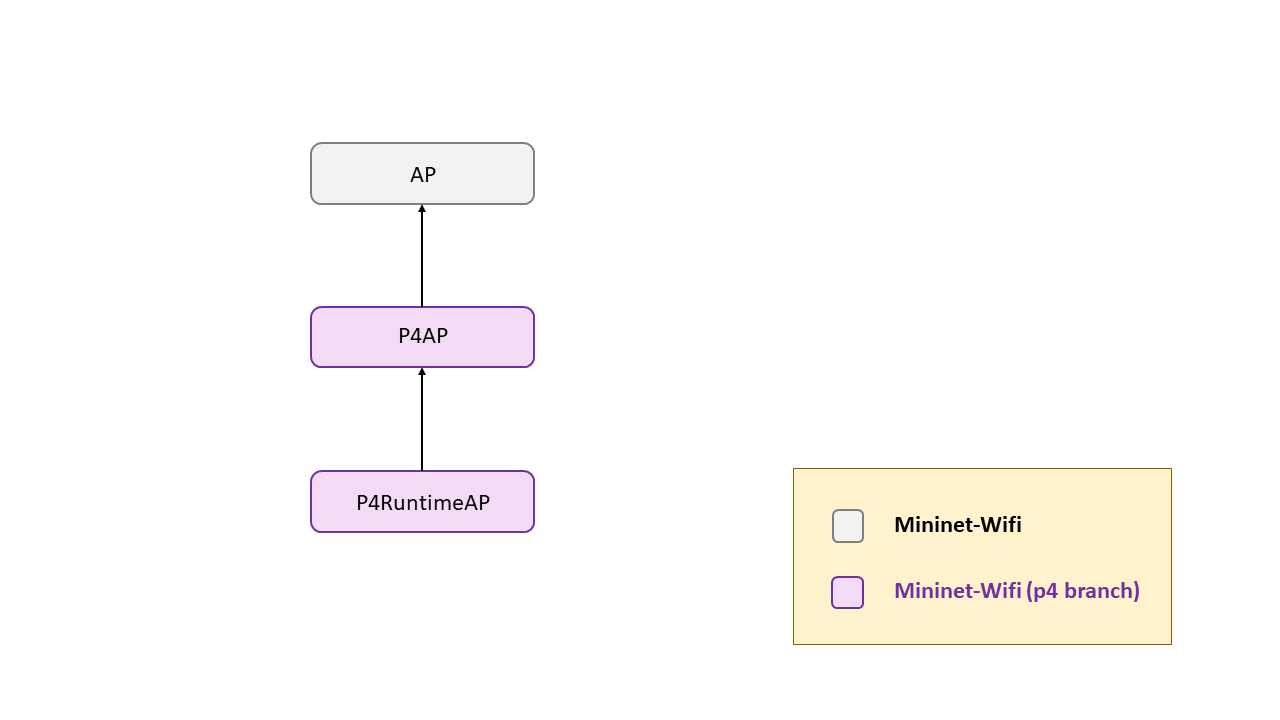
\includegraphics[width=15.5cm]{archivos/img/dev/p4-wifi/analysis/p4_Mininet_Wifi_UML.png}
    \caption{UML de la integración BMv2 - Mininet-WiFi}
    \label{fig:analysis_p4_wifi_9}
\end{figure}

Además debatiendo con Ramon Fontes sobre la implementación de estas clases,  indicó que sería de gran utilidad que dichas clases tuvieran soporte de ejecución en Network Namespaces, por lo que de forma paralela se tuvo que crear una clase llamada \texttt{Netns\_mgmt}\footnote{\url{https://github.com/davidcawork/TFG/tree/master/src/netns_mgmt}}. Esta clase ayudará a gestionar la ejecución de código Python en \textit{runtime} en una Network namespace indicada haciendo uso de la llamada al sistema \textbf{setns} la cual asocia el procesos sobre la cual se realiza esta llamada, a una \textit{Namespace} indicada.\\
\par

Con la ayuda de esta clase, \texttt{Netns\_mgmt}, se pudo conseguir configurar cada \gls{bmv2} en su propia \textit{Network Namespace}, por lo que la integración se dio por terminada. Adicionalmente se añadieron dos ejemplos a Mininet-WiFi con la finalidad de ayudar a las personas que vayan hacer uso de clase. Dichos ejemplos pueden ser encontrados \href{https://github.com/davidcawork/mininet-wifi/tree/p4/examples/p4}{\textbf{aquí}}.\footnote{\url{https://github.com/davidcawork/mininet-wifi/tree/p4/examples/p4}}\\
\par
Todo este desarrollo se llevo a cabo en un fork de Mininet-WiFi, y dentro de este en una rama en particular, en la cual se llevan a cabo todos los desarrollos de P4. Una vez finalizada la integración, se ofreció el desarrollo al repositorio oficial de Mininet-WiFi vía pull-request. Actualmente se ha dejado a la espera de hacer un \textit{upgrade} a las dependencias donde fue llevada a cabo la integración, ya que Mininet-WiFi está trabajando con las últimas versiones. En cambio, para el desarrollo de los casos de uso P4-wireless, se hará uso de las últimas versiones  estables de las dependencias del entorno P4.

\vspace{1cm}
\textbf{Puesta en marcha del Mininet-WiFi modificado}\\
\par
\label{mn_wifi_own_deps}

Para poder probar el desarrollo llevado a cabo con Mininet-WiFi se deberán seguir los pasos indicados en el bloque \ref{code:wifi_bmv2_integration_deps} previamente. Se deberá bajar el repositorio del fork de Mininet-WiFi. Se hará un checkout para moverse desde la rama master del repositorio a la rama de desarrollo de elementos P4.

\begin{lstlisting}[language= bash, style=Consola, caption={Instalación de Mininet-WiFi modificado},label=code:wifi_bmv2_integration_deps]
    # Se descarga el repositorio
    git clone https://github.com/davidcawork/mininet-wifi
    
    # Se adquieren las etiquetas y se cambia de rama
    cd mininet-wifi && git fetch
    git checkout p4
    
    # Se "recompilará" Mininet-Wifi
    sudo make install
\end{lstlisting}
\vspace{0.5cm}

Como la rama de desarrollo añade módulos nuevos a Mininet-WiFi se deberá ``recompilar" de nuevo haciendo un make install desde el directorio \texttt{/mininet-wifi}. Para que los módulos añadidos funcionen correctamente se deberán tener las dependencias del entorno P4, en la tabla \ref{tab:mn-wifi_bmv2_integration_deps} se pueden comprobar que versiones son requeridas.\\
\par

\begin{table}[ht]
\centering

\begin{tabular}{|c|c|}
\hline
\rowcolor[HTML]{EFEFEF} 
{\color[HTML]{24292E} \textbf{Dependencia}} & {\color[HTML]{24292E} \textbf{Versión requerida}} \\ \hline
\href{https://github.com/p4lang/behavioral-model}{\textbf{BMV2}}                                        & \texttt{b447ac4c0cfd83e5e72a3cc6120251c1e91128ab}          \\ \hline
\href{https://github.com/p4lang/PI}{\textbf{PI}}                                          & \texttt{41358da0ff32c94fa13179b9cee0ab597c9ccbcc}          \\ \hline
\href{https://github.com/p4lang/p4c}{\textbf{P4C}}                                         & \texttt{69e132d0d663e3408d740aaf8ed534ecefc88810}         \\ \hline
\href{https://github.com/protocolbuffers/protobuf}{\textbf{PROTOBUF}}                                    & \texttt{v3.2.0}                                        \\ \hline
\href{https://github.com/grpc}{\textbf{GRPC}}                                        & \texttt{v1.3.2}                                           \\ \hline
\end{tabular}%
\caption{Resumen de las versiones requeridas de la interfaz BMv2 - Mininet-WiFi}
\label{tab:mn-wifi_bmv2_integration_deps}
\end{table}

